\documentclass[a4paper, 12pt, final, garamond]{book}
\usepackage{cours-preambule}

\raggedbottom

\makeatletter
\renewcommand{\@chapapp}{M\'ecanique -- chapitre}
\makeatother

\begin{document}
\setcounter{chapter}{3}

\chapter{TD application~: approche \'energ\'etique}

\section{Intérêt des raisonnements énergétiques}
\begin{enumerate}
    \item On lance une balle avec une vitesse initiale $v_0$ vers le haut depuis
        l'altitude $z = 0$. Déterminer la hauteur maximale atteinte par la balle
        en négligeant tout frottement.
    \item On considère un pendule simple (masse $m$ ponctuelle, longueur $\ell$,
        pas de frottements). On fait partir ce pendule de la verticale ($\tt =
        0$, en bas) en lui communiquant une vitesse initiale $v_0$. Déterminer
        l'expression de l'amplitude maximale $\tt_{\max}$ du mouvement.
\end{enumerate}

\section{Curling}
Le curling est un sport de précision pratiqué sur la glace avec des pierres en
granite, taillées et polies selon un gabarit international. Le but est de placer
les pierres le plus près possible d'une cible circulaire dessinée sur la glace,
appelée la maison. \bigbreak

\begin{minipage}{0.60\linewidth}
    Nous envisageons le lancer d'une pierre assimilée à un point M de masse $m =
    \SI{20}{kg}$ glissant selon l'axe O$x$ vers le point M$_0$ visé (la maison).
    La pierre est lancée de la position initiale O avec une vitesse $\vfo =
    v_0\ux$, la maison se trouvant à la distance $D = {\rm OM_0} = \SI{25}{m}$
    du point O.
\end{minipage}
\hfill
\begin{minipage}{0.35\linewidth}
    \begin{center}
        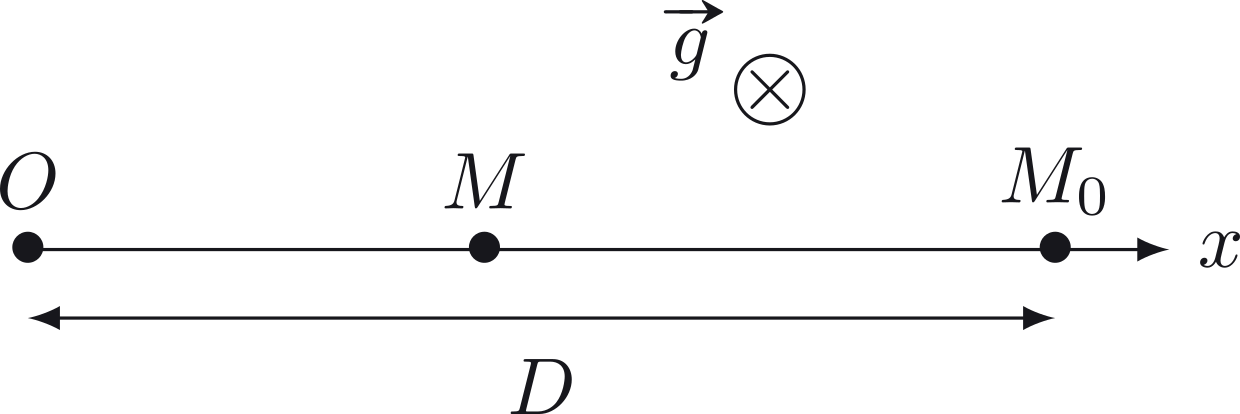
\includegraphics[width=\linewidth]{curling_plain}
    \end{center}
\end{minipage} \bigbreak

Nous supposerons que la force de frottement solide $\Ff = -F_0\ux$ de la glace
sur la pierre est constante pendant toute la glissade et s'annule lorsque la
vitesse de la pierre s'annule. Nous prendrons $F_0 = \SI{3.0}{N}$. Nous
négligerons par ailleurs toute force de frottement fluide.

Le lancer étudié est supposé gagnant~: la pierre atteint la maison et s'y
arrête. \bigbreak

\begin{enumerate}
    \item Que valent les énergies cinétiques initiale $\Ec_{c,I}$ et finale
        $\Ec_{c,F}$ de la pierre ?
    \item Calculer le travail des forces appliquées sur la pierre pendant la
        glissade.
    \item Appliquer le théorème de l'énergie cinétique à la pierre et en déduire
        la vitesse initiale $v_0$.
\end{enumerate}

\section{Piégeage d'un électron}
Considérons le mouvement selon un axe (O$z$) d'un électron de masse $m =
\SI{9.1e-31}{kg}$ et de charge $-e = \SI{-1.6e-19}{C}$ dans un dispositif de
piégeage. Il est soumis uniquement à des forces conservatives, d'énergie
potentielle totale $\Ec_p(z)$ telle que~:
\[\Ec_p(z) = \frac{eV_0}{2d^2}z^2\]
avec $V_0 = \SI{5.0}{V}$ et $d = \SI{6.0}{mm}$. \bigbreak
\begin{enumerate}
    \item Tracer l'allure de $\Ec_p(z)$. Identifier la position d'équilibre et
        donner sa stabilité.
    \item Calculer la fréquence des oscillations de l'électron dans le piège.
    \item Exprimer la résultante des forces $\Ff$ sur l'électron. On rappelle
        qu'en coordonnées cartésiennes, on a
        \[\gd{f}(x,y,z) = \pdv{f}{x}\ux + \pdv{f}{y}\uy + \pdv{f}{z}\uz \]
\end{enumerate}

\section{Balle dans un tonneau}
\begin{minipage}{0.60\linewidth}
    Une balle, assimilée à un point matériel M de masse $m$, est lâchée sur une
    rampe sans vitesse initiale depuis le point A d'une hauteur $h$ par rapport
    au point O le bout de la rampe. Elle achève sa course dans un tonneau
    circulaire de rayon $R$ lui permettant éventuellement de faire des
    \textit{loopings}. On néglige les frottements.
\end{minipage}
\hfill
\begin{minipage}{0.35\linewidth}
    \begin{center}
        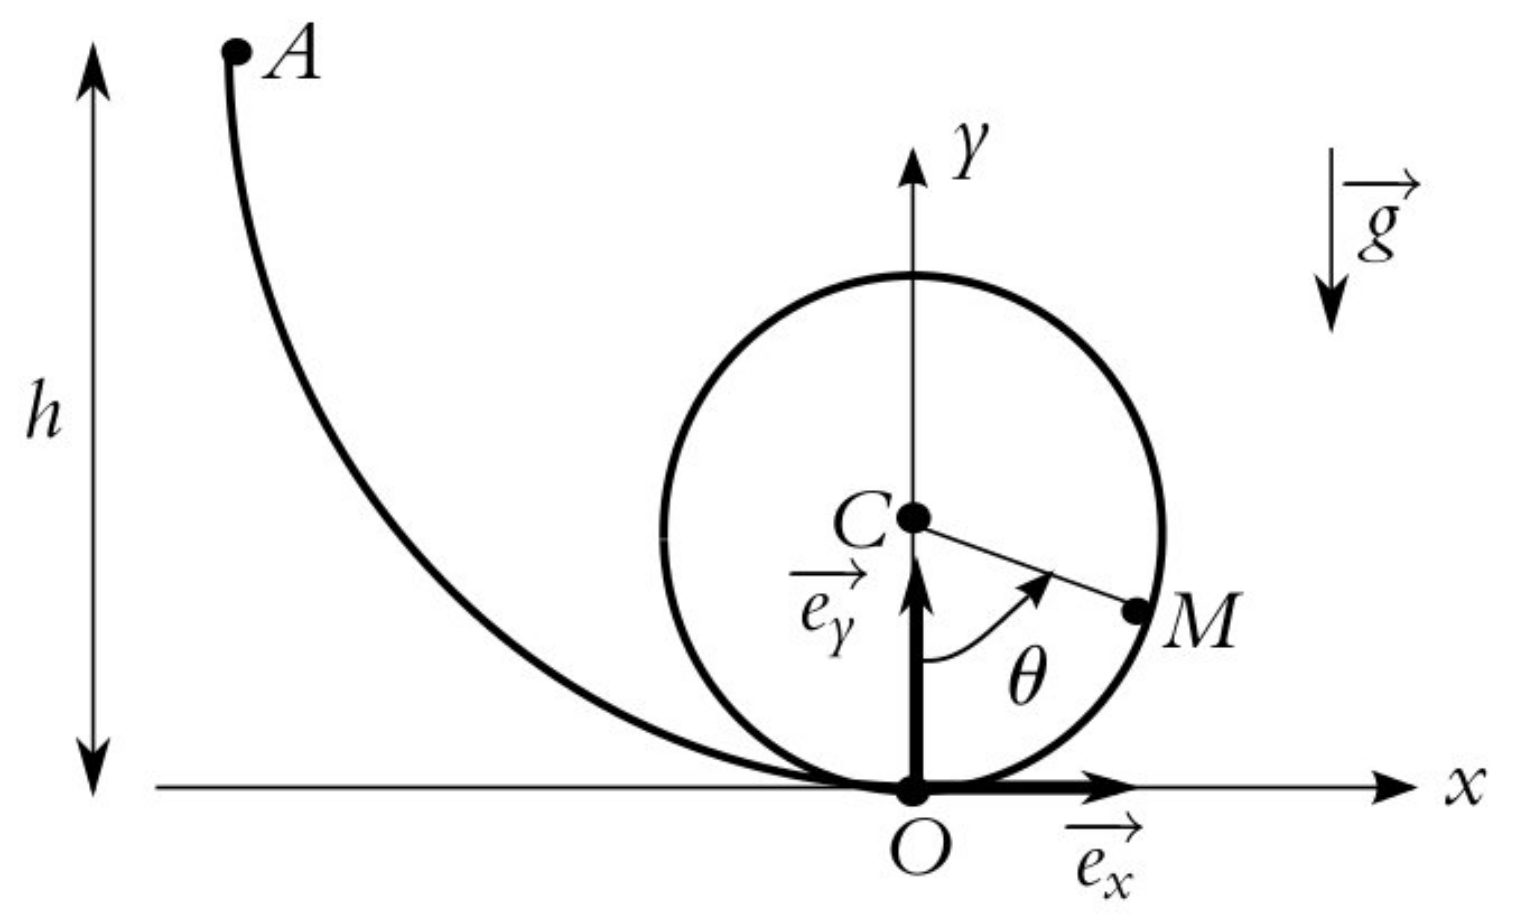
\includegraphics[width=\linewidth]{bille_tonneau-plain}
    \end{center}
\end{minipage}

\begin{enumerate}
    \item Exprimer la norme $v_\Or$ de la vitesse en O, puis $v_\Mr$ en un point
        M quelconque du tonneau repéré par l'angle $\tt$, en fonction de $g$,
        $h$, $a$ et $\tt$. Donner la relation entre $v_\Mr$ et $\tp$.
    \item Déterminer la réaction du tonneau en un point du cercle en fonction de
        $g$, $h$, $a$ et $\tt$.
    \item Déterminer la hauteur minimale $h_{\min}$ pour que la bille fasse le
        tour complet du tonneau sans tomber.
\end{enumerate}

\end{document}
